\begin{figure}[h]
\centering
	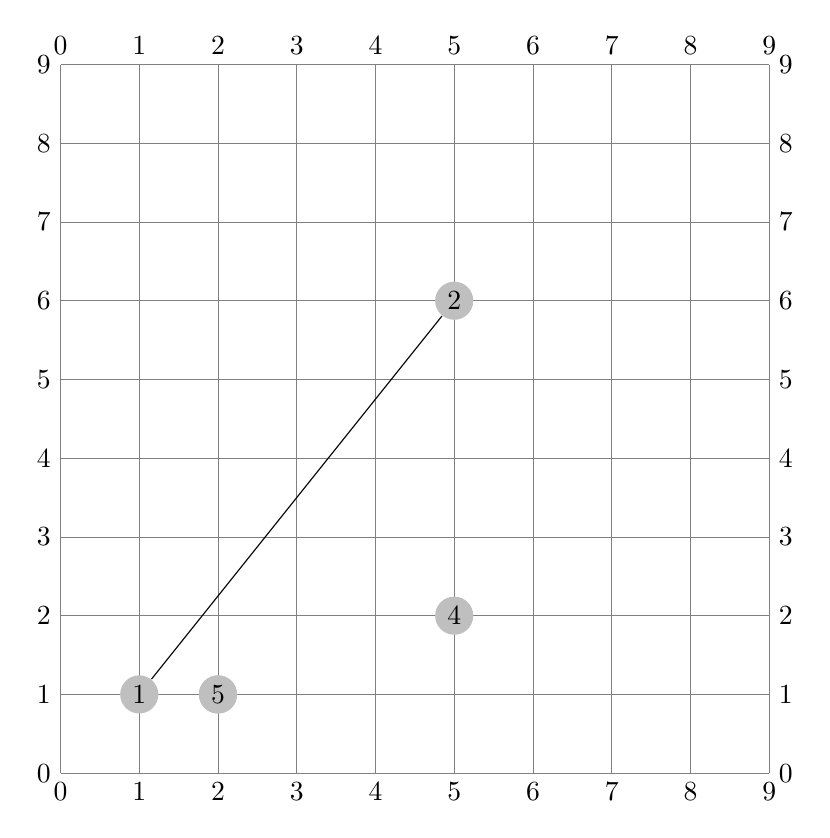
\begin{tikzpicture}
		\draw[help lines] (0,0) grid (9,9);
		\foreach \x in {0,...,9}{
			\draw(0,\x) node[anchor=east]{\x};
			\draw(9,\x) node[anchor=west]{\x};
			\draw(\x,0) node[anchor=north]{\x};
			\draw(\x,9) node[anchor=south]{\x};
		}
		\tikzstyle{vertex}=[circle,fill=black!25,minimum size=12pt,inner sep=2pt]
		\node[vertex] (g_1) at (1,1) {1};
		\node[vertex] (g_2) at (5,6) {2};
		\node[vertex] (g_3) at (2,1) {3};
		\node[vertex] (g_4) at (5,2) {4};
		\node[vertex] (g_5) at (2,1) {5};
		\draw (g_1) -- (g_2);
	\end{tikzpicture}
\end{figure}


\begin{figure}[h]
\centering
	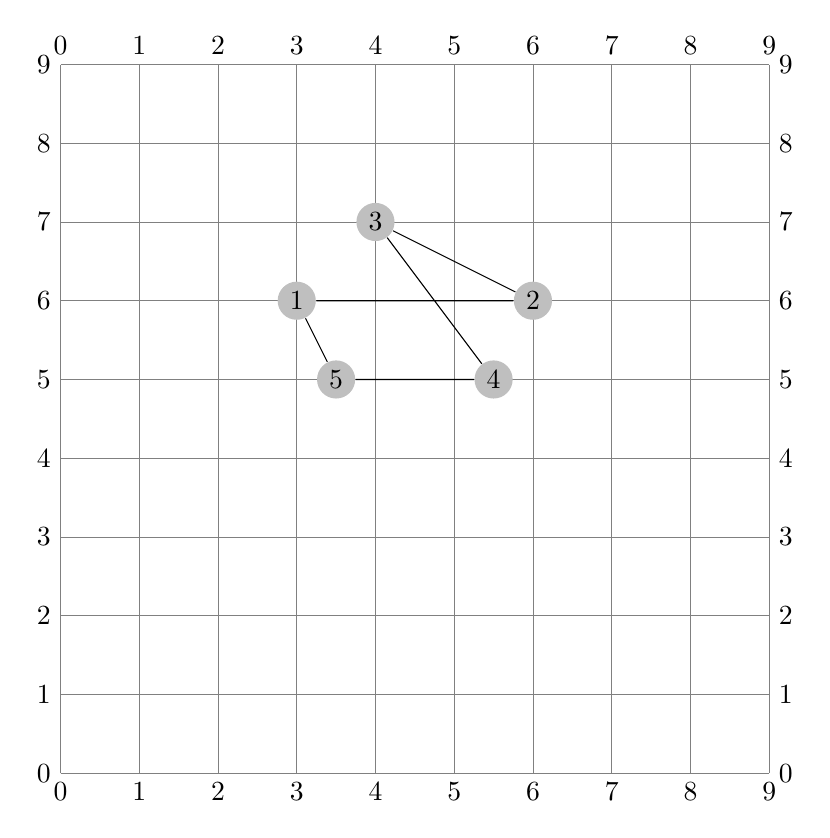
\begin{tikzpicture}
		\draw[help lines] (0,0) grid (9,9);
		\foreach \x in {0,...,9}{
			\draw(0,\x) node[anchor=east]{\x};
			\draw(9,\x) node[anchor=west]{\x};
			\draw(\x,0) node[anchor=north]{\x};
			\draw(\x,9) node[anchor=south]{\x};
		}		\tikzstyle{vertex}=[circle,fill=black!25,minimum size=12pt,inner sep=2pt]
		\node[vertex] (g_1) at (3,6) {1};
		\node[vertex] (g_2) at (6,6) {2};
		\node[vertex] (g_3) at (4,7) {3};
		\node[vertex] (g_4) at (5.5,5) {4};
		\node[vertex] (g_5) at (3.5,5) {5};
		\draw (g_1) -- (g_2) -- (g_3) -- (g_4) -- (g_5) -- (g_1) -- cycle;
	\end{tikzpicture}
\end{figure}

